\chapter{Einleitung}
Der technologische Fortschritt in der medizinischen Bildgebung hat dazu geführt, dass es heute in der klinischen Diagnostik selbstverständlich ist, innerhalb weniger Minuten den kompletten Patienten  mit hoher Auflösung und hohem Kontrast abzubilden.
Dabei spielt die \gls{mrt} nicht nur für die morphologische, sondern auch für die funktionelle oder diffusionsgewichtete Bildgebung eine entscheidende Rolle. Gegenüber anderen Verfahren, auch \textit{Modalitäten} genannt, bietet die \gls{mrt} zahlreiche Vorteile: Es entstehen Schnittbilder, die mit einem sehr hohen Weichteilkontrast einen (schattenfreien) Einblick in den Körper liefern. Im Gegensatz zur \gls{ct} kommt dabei keine ionisierende Strahlung zum Einsatz: Statt die Abschwächung von Röntgenstrahlung durch den Körper zu messen, wird der \gls{nmr}-Effekt von Wasserstoffprotonen im Körper genutzt. Durch die verschiedenen möglichen Bildgewichtungen, wie zum Beispiel nach der Protonendichte oder nach der longitudinalen Relaxationszeit der Protonen-Spins und die zahlreichen möglichen Pulssequenzen, kann mehr auf den Bildentstehungsprozess als beim Röntgen und bei der \gls{ct}. Dadurch kann oft auf ein Kontrastmittel verzichtet werden.

Die Entwicklungen in der klinischen Bildgebung wirken sich auch positiv auf den Sektor der \textit{präklinischen Bildgebung} (eng. preclinical imaging) aus. Durch die inzwischen möglichen, sehr hohen Auflösungen und kurze Aufnahmezeiten ist die Abbildung von Kleintieren, wie Mäusen, Ratten oder anderen Nagern, in ausreichender Qualität möglich (vgl. \autoref{fig:fortschritt}). Präklinische Systeme sind gezielt auf die Größe der Tiere und den Einsatz in der Forschung optimiert.

\begin{figure}[H]
	\centering
	\subcaptionbox[Erste MRT-Aufnahme]{Eine der ersten \gls{mrt}-Aufnahmen eines lebendigen Menschens; 1977; Farbe kodiert Signalstärke; \cite{damadian1977}}{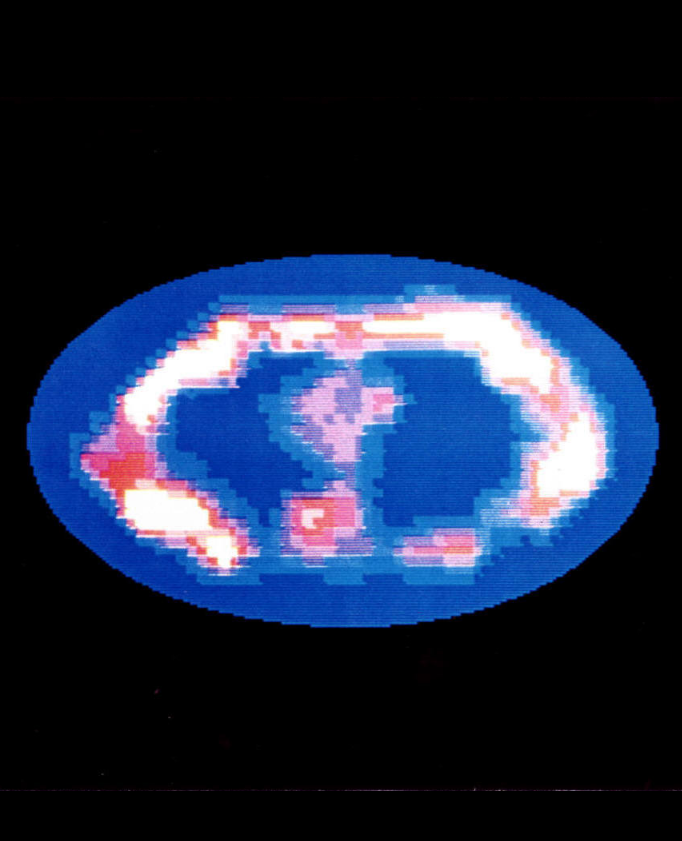
\includegraphics[width=0.4\textwidth]{img/fonarImage.PNG}}
	\hfill
	\subcaptionbox[Hochauflösende MRT Aufnahme einer Maus]{Hochauflösende \gls{mrt}-Aufnahme einer Maus; 2013;  \cite{rascheUlm}}{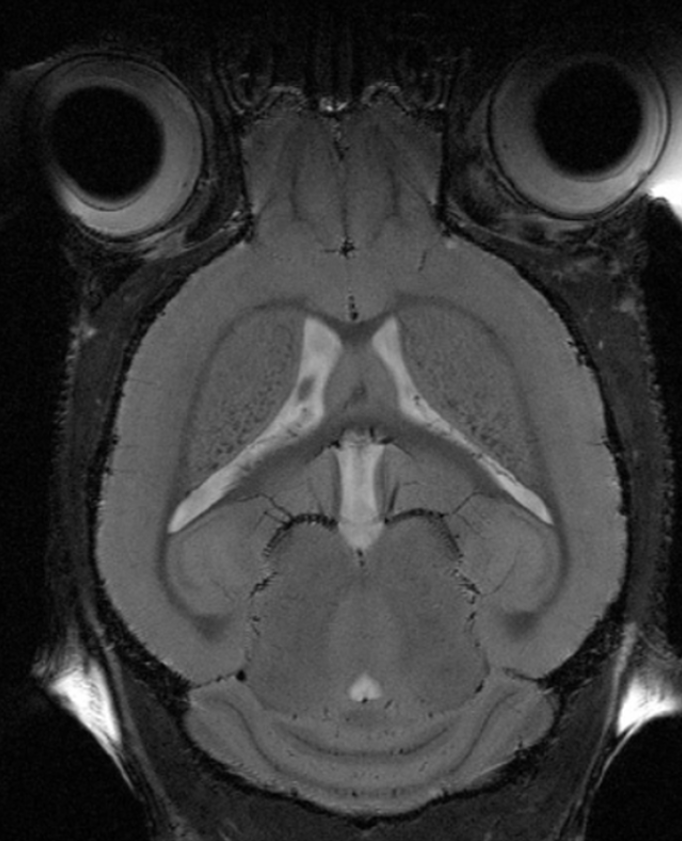
\includegraphics[width=0.4\textwidth]{img/mouseBrain.PNG}}
	\caption{Fortschritt in der \gls{mr}-Bildgebung 1977 bis 2013}
	\label{fig:fortschritt}
\end{figure}

Präklinische Abbildungssysteme werden meist in der Forschung oder bei der Entwicklung von Medikamenten eingesetzt. Dort liefern Tierversuche wichtige Erkenntnisse in der Neurologie, Onkologie oder für den Nachweis der Wirksamkeit neu entwickelter Präparate. Die Nutzung moderner Tomographen entspricht dabei nicht nur den Richtlinien von \textit{3R} \cite{Russell1992}, sondern erleichtert gegenüber klassisch-invasiven Techniken auch die zeitabhängige Verfolgung von Prozessen in den Tier-Modellorganismen. Klassisch wäre eine große Anzahl an Versuchstieren nötig, da z.B. das Wachstum eines Tumors einer statistischen Verteilung folgt. Dadurch, dass mit präklinischen \gls{mrt}s das Wachstum eines Tumors in \emph{einem} Tier verfolgt werden kann, ist das Tier sein eigener Kontrollversuch, wodurch die Zahl der Versuchstiere reduziert und die Aussagekraft der Studien verbessert werden können \cite{Bradley2013}.

Im Segment der präklinischen Bildgebung ist die (mikro) \gls{mrt} die wichtigste Modalität. Bruker BioSpin ist auf dem Markt der präklinischen Bildgebungssysteme Marktführer. Die wichtigsten Mitbewerber sind \textit{Aspect Imaging} und \textit{Mediso}.
 
\section{Ausgangssituation und Aufgabenstellung}
In einer typischen Konfiguration eines Bruker \gls{mr}-Tomographens werden ein \gls{rf}-Sendekanal und mehrere \gls{rf}-Empfangskanäle verwendet. Übliche \gls{mrt} Prozeduren in der präklinischen Bildgebung nutzen vier oder mehr Empfangsspulen. In der \gls{nmr}-Spektrometrie wird eine gleiche Anzahl an Sende- und Empfangsspulen eingesetzt.

Aktuell teilen sich die Bruker \gls{nmr}-Spektrometer der \textit{AVANCE NEO} Generation und \gls{mr}-Tomographen der \textit{BioSpec}-Linie große Teile der Hochfrequenz-Elektronik. Sende- und Empfangselektronik für die in der Magnetresonanz-Technik notwendigen \gls{rf} Pulse mit Frequenzen von \SI{40}{\mega\hertz} bis einigen hundert \SI{}{\mega\hertz} sind auf Steckkarten für modulare Chassis-Systeme untergebracht. Dabei besteht eine Steckkarte (TRX1200, siehe \autoref{fig:trx12004er}) immer aus einem Sendepfad mit allen nötigen Wandlern und Verstärkern und einem Empfangspfad mit Eingangsverstärkern und den \gls{adc}.

\begin{figure}[H]
	\centering
	\resizebox{0.6\textwidth}{!}{\includegraphics[]{img/trx1200mult.tikz}}
	\caption[Bruker Avance Neo TRX1200 Karte]{AV4 TRX1200 (verwendet in Bruker Avance Neo \gls{nmr} Spektrometer und einigen \gls{mr}-Tomographen)}
	\label{fig:trx12004er}
\end{figure}

Kommt eine solche Anordnung in der \gls{mrt} zum Einsatz, ergibt sich eine Situation wie in \autoref{fig:trx12004er} angedeutet: Bei vier notwendigen Karten wird lediglich eine voll ausgenutzt. Bei den restlichen TRX1200 Karten bleibt die Sendeelektronik ungenutzt.

Für zukünftige Produktentwicklungen sollen vorab in einem Technologie\-projekt Möglich\-keiten zur Optimierung der Signalkette evaluiert werden. Dabei spielen neben technischen Optimierungsmöglichkeiten auch wirtschaftliche Aspekte eine Rolle.
Durch die unterschiedlichen Qualitätsanforderungen an die Sende- und Empfangselektroniken in der \gls{nmr} und der \gls{mrt} ergibt sich ein Einsparpotential: Da in der \gls{nmr} Spektren über die Fouriertransformation des \gls{fid} gemessen werden, ist zum Erreichen einer hohen spektralen Auflösung aufgrund der Reziprozität von Zeit- zu Frequenzbereich eine lange Messzeit\footnote{Bis hin zu mehreren Stunden} notwendig. An das Taktsignal des, zur Digitalisierung des \gls{fid}s, genutzten \gls{adc} werden daher hohe Stabilitätsanforderungen gestellt. In der \gls{mrt} dauert die Aufnahme eines Empfangssignals (in der Regel kein \gls{fid}, sondern ein Echo) meist nur wenige Millisekunden. Die Zeitdauern sind bei der klassischen \gls{mrt} zur morphologischen Bildgebung durch die verschiedenen eingesetzten Pulssequenzen, die gewünschte Ortsauflösung, etc. bestimmt.
Durch die kürzere Akquisitionszeit einer \gls{mrt}-Aufnahme im Vergleich zu einem \gls{nmr}-Spektrum werden weniger strenge Anforderungen bezüglich der zeitlichen Langzeitstabilität an den Referenzoszillator gestellt.

Zur Charakterisierung der Einflüsse eines weniger stabilen Oszillators und anderer potenziell negativer Einflüsse auf die \gls{mr}-Signale soll eine Simulation eingesetzt werden. Statt die komplette Signalkette auf der Ebene der einzelnen elektronischen Baugruppen durchzurechnen wird zunächst auf einer höheren Abstraktionsebene angesetzt. In einer Simulation, beginnend von einer dreidimensionalen Eingangsmatrix, werden Schichtbilder simuliert, wie sie auch ein \gls{mr}-Tomograph erzeugen würde. Dazu müssen die Vorgänge, wie sie im echten Gerät ablaufen, nur in soweit modelliert werden, wie sie für die zu untersuchende Störung relevant sind. Da in dieser Arbeit der Einfluss von Phasenrauschen des Referenzoszillators und damit des \gls{adc}-Taktsignals in Abhängigkeit verschiedener \gls{mrt}-Pulssequenzen untersucht werden soll, ist es für die Simulation erforderlich, verschiedene Pulssequenzen abfahren zu können und das \gls{rf}-Empfangssignal gezielt zu manipulieren.

Für numerische Simulationen in den Natur- und Ingenieurwissenschaften ist das Programmpaket \textit{MATLAB}\cite{matlab} von \textit{The MathWorks} weit verbreitet. Es existieren einige Ver\-öffent\-lichungen zu \gls{mrt}-Simulationen in MATLAB\footnote{zum Beispiel \cite{Kern2012}}, in denen sich die Autoren meist auf die Simulation bestimmter Teilaspekte der \gls{mrt} beschränken. Mehr auf eine vollständige Simulation ausgerichtet ist das Programm \textit{\gls{mr}iLab}\cite{Liu2017} (siehe \autoref{fig:mrilabscreenshot}).

In dieser Arbeit soll unter anderem \gls{mr}iLab auf die Eignung als Simulationsumgebung für kommende Entwicklungstätigkeiten bei Bruker BioSpin hin untersucht werden. Im weiteren Verlauf der Arbeit wird Phasenrauschen aus theoretischen Überlegungen, Datenblättern und realen Messungen simuliert und die Einflüsse von diesem auf die Bildqualität der rekonstruierten MR-Bilder untersucht.


